%%%%%%%%%%%%%%%%%%%%%%%%%%%%%%%%%%%%%%%%%%%%%%%%%
% Relatório Final - Projeto de Pesquisa
% Métodos de Otimização
% Baltz & Machado
% Capítulo 1
%%%%%%%%%%%%%%%%%%%%%%%%%%%%%%%%%%%%%%%%%%%%%%%%%


\chapter{\Large{Métodos Matemáticos de Otimização}}\label{chp:1}


\section{{O Conceito de Otimização}}

\hspace{0.8cm}
Diz-se otimização, o processo que tem como objetivo encontrar condições que
minimizam ou maximizam algo (seja energia, tempo, dinheiro, etc). Sendo este,
muitas vezes um trabalho árduo, custoso.

Dessa maneira, na matemática, este processo é amplamente utilizado quando
busca-se valores pertencentes ao conjunto \textit{A} (que pode ter
restrições), com o objetivo de encontrar uma solução ótima, aplicando os valores
de \textit{A} em numa função objetivo predefinida.

Podendo assim, ser representada da seguinte forma:

    Dada a função
        \begin{equation}
            f : A \rightarrow \mathbb{R}
        \end{equation}

        \begin{itemize}
                \item Maximização pode ser definida como:
        \end{itemize}

                busca pelo elemento \(x_0 \in A\), que satisfaz:

                    \begin{equation}
                        f(x_0) \geq f(x);
                    \end{equation}

                para todo \(x \in A\).

        \begin{itemize}
                \item Minimização pode ser definida como:
        \end{itemize}

                busca pelo elemento \(x_0 \in A\), que satisfaz:

                    \begin{equation}
                        f(x_0) \leq f(x);
                    \end{equation}

                para todo \(x \in A\).

\vspace{\baselineskip}
Com isso, podemos agora entender como esse processo pode ser custoso. Iniciando
com fato de que existem os pontos máximos e mínimos (pontos críticos), locais
e globais, no espaço das funções. Sendo os pontos críticos locais, aqueles que
não são os menores ou maiores valores para a minimização e maximização,
respectivamente. E os pontos globais, aqueles que representam o menor ou maior
valor no espaço das funções, para a minimização e maximização, respectivamente.

Criando assim, uma certa incerteza ao encontrar um valor crítico numa função,
já que é estritamente difícil saber se o ponto crítico encontrado é local ou
global. Como pode-se perceber na Figura
\ref{grafico_local_global_pontosCriticos}.


\begin{figure}[h]
    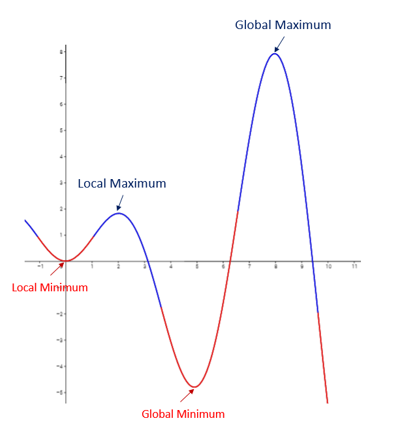
\includegraphics[width=0.43\textwidth]
        {src/grafico_local_global_pontosCriticos.png}
    \centering
    \caption{Exemplo de pontos críticos locais e globais indicados no gráfico
        de uma função}
    \label{grafico_local_global_pontosCriticos}
\end{figure}


\section{{Otimização de Funções à Uma Variável Real}}

\hspace{0.8cm}

Evidente que funções possuem as variáveis dependentes (a qual representa o
objeto da otimização) e variáveis independentes (cujo suas grandezas podem ser
selecionadas), podemos denotar que, para a equação

\begin{equation}
	y = f(x),
\end{equation}
quando buscamos otimizá-la, temos como objetivo encontrar valores que quando
aplicados à \textit{x}, temos o mínimo ou máximo valor \textit{y} (seja ele
local, ou preferencialmente global).

Partindo dessa perspectiva, acaba surgindo a necessidade de utilizar algum
recurso para encontrar o os pontos críticos. E nesse sentindo, pode-se utilizar
a técnica de \textbf{derivação}, donde, oferece como recurso a possibilidade de
identificar tais pontos.

A derivada é a representação da taxa de variação de uma função, em relação a
um ponto. A partir daí, podemos observar um fator interessante; por exemplo,
quando a função está num ponto máximo, existem duas possibilidades, a primeira,
sendo a função parando de crescer e em seguinda se tornando indefinida; e a
segunda possibilidade quando a função para de crescer e começa a decrescer.
Com isso, é importante ressaltar que por definição, quando a derivada (taxa de
variação) em um ponto é positiva, a função cresce, e quando negativa a função
decresce. Conclui-se que, quando a derivada que representa a taxa de variação é
zero, a função ou para de crescer ou de decrescer, sendo assim um
ponto de máximo ou de mínimo.

Com o uso da derivada, podemos pensar num método de otimização bastante simples,
considerando \(f(x)\) a função que queremos otimizar e \(f'(x)\) sua função
derivada, podemos dizer que o conjunto $O$ possui todos os ótimos locais e
globais de \(f(x)\):

\begin{equation}
    O := \{f(x) | f'(x) = 0\}
\end{equation}


Portanto, aplicando um filtro em $O$ para obeter o máximo e mínimo do conjunto,
acabamos por obeter o máximo e mínimo de \(f(x)\):


\begin{equation}
    max(f(x)) = max(O)
\end{equation}

\begin{equation}
    min(f(x)) = min(O)
\end{equation}


Então podemos perceber dois problemas, determinar como encontrar os pontos onde
a derivada se anule, e determinar se temos de fato todos os pontos.

Desconsiderando por agora o problema de determinar se tem-se todos os pontos
críticos. Vamos considerar então o problema de encontrar os pontos críticos,
levando em conta boas aproximações.

O Método de Newton nos diz que uma sequência \(\{x_k\}\) converge para o mínimo
de \(f(x)\):

\begin{equation}
    x_{k+1} = x_{k} - \frac {f'(x_{k})}{f''(x_{k})}
\end{equation}

O que este método faz de fato é encontrar zeros de uma função \(g(x)\) a partir
da mesma sequência \(\{x_k\}\), afim de que \(x_k\) converga para uma entrada
\(x^*\) de \(g(x)\), tal que a mesma se anule:

\begin{equation}
    x_{k+1} = x_{k} - \frac {g(x_{k})}{g'(x_{k})}
\end{equation}

\begin{equation}
    g(x^*) = 0
\end{equation}


Com isso temos um método que minimiza uma função que pode ser derivada duas
vezes (caso não possa, aproximações de suas primeiras e segundas derivadas
podem ser boas o suficiente) a partir de um valor de entrada. O método é
simples, entrega muitas vezes ótimos locais próximos ao ponto inicial, mas tem
seu destaque pode ser curto e facilmente computável.

Problemas de maximização podem ser vistos sob o seguinte olhar:

\begin{equation}
    max(f(x)) = min(-1 * f(x))
\end{equation}

Que com isto podem ser otimizados pelo Método de Newton também.

O movimento de \(x_k\) dentro da sequência, é determinado pela relação das
quantidades e propriedades que tanto a primeira quanto a segunda derivada
oferecem. As quantidades determinam a velocidade do motivento, e os sinais
indicam a direção do movimento. De certa forma podemos ver esse movimento da
sequência \(\{x_k\}\) como instantes do movimento de uma bola numa ladeira, que
no começo de sua descida é acelerada, e, conforme chega ao plano no fim da
ladeira, começa a reduzir sua velocidade, até supostamente chegar no ponto mais
baixo.

\section{{Programando o Método}}

\hspace{0.8cm}

A forma mais simples e mais util de implementar o metodo de Newton é na forma
de busca das raizes, que uma vez  implementada, só precisamos por como entrada
a priemira e a segunda derivada da função que desejamos minimizar, já que o
método não precisa saber qual a função de fato. A seguir temos a implementação
na liguagem de programação Rust:

\begin{lstlisting}
pub fn newton1x1<F>(funcao_derivada: &F, x: f64) -> (usize, f64)
where
    F: Fn(f64) -> f64,
{
    let mut entrada_atual = x;
    let maximo_iteracoes = 100;

    for iteracao_atual in 1..=maximo_iteracoes {
        let diferenca: f64 =
            funcao_derivada(entrada_atual.clone())
            /
            derive1x1(&funcao_derivada, &entrada_atual);

        println!("diferenca: {}", diferenca);
        entrada_atual -= diferenca;

        if diferenca.abs() < 0.0000001 {
            return (iteracao_atual, entrada_atual);
        }
    }

    return (maximo_iteracoes, entrada_atual);
}
\end{lstlisting}


Os parametros da função são:

    \begin{itemize}
            \item Uma função \(f : \mathbb{R} \rightarrow \mathbb{R}\)
            \item Uma entrada x sendo o chute inicial do otimo.
    \end{itemize}


A função derive1x1 recebe como parametro uma função e um ponto, tendo como
retorno a derivada da função entregue, no ponto especificado. Restingindo-se
à funções do tipo \(f : \mathbb{R} \rightarrow \mathbb{R}\), donde deve ser
escrita pelo úsuario como bem entender.



\textcolor[rgb]{1,0,0}{\section{{Otimização de Funções à Várias Variáveis}}}

\hspace{0.8cm}





%
